\section{Assumptions of survival analysis}

%----------------------------------------------------------------------
\begin{frame}{Common assumptions in survival analysis}
    \begin{enumerate}
      \item Subjects are \textbf{either} ``healthy'' \textbf{or} ``diseased'', with
	no intermediate state.
      \item The disease is \textbf{irreversible}, or requires intervention
	to be cured.
      \item The time of disease incidence is known \textbf{exactly}.
      \item The disease is \textbf{accurately} diagnosed.
    \end{enumerate}
    \pause
    These assumptions are true for \alert{death} and many
    \alert{chronic diseases}.
\end{frame}

%----------------------------------------------------------------------
\begin{frame}{Is the disease a dichotomy?}
  A disease may be preceded by a \alert{sub-clinical} phase before it shows
  symptoms.
  \pause
  \begin{center}
    \begin{tabular}{ll}
      {\bf AIDS} & Decline in CD4 count \\
      {\bf Cancer} & Pre-cancerous lesions \\
      {\bf Type 2 Diabetes} & Impaired glucose tolerance \\
    \end{tabular}
  \end{center}
  \pause
  Or a disease may be classified into \alert{degrees of severity}
  (mild, moderate, severe).
\end{frame}

%----------------------------------------------------------------------
\begin{frame}{A model for cervical cancer}
  Invasive squamous cell cancer of the cervix is preceded by
  cervical intraepithelial neoplasia (CIN)\\[-1ex]
\hspace*{-2em}
\includegraphics[width=1.15\textwidth,keepaspectratio]<1| handout:0>{cervical2}
\includegraphics[width=1.15\textwidth,keepaspectratio]<2| handout:0>{cervical3}
\includegraphics[width=1.15\textwidth,keepaspectratio]<3| handout:1>{cervical4}\\[-1ex]
The purpose of a screening programme is to detect and treat CIN.

\onslide<2->{Aim of the modeling the \alert<2>{transition rates}
  between \alert<3>{states},
  is to be able predict how population moves between \alert<3>{states}}

\onslide<3->{Probabilities of \alert<3>{state} occupancy can be calculated.}

\end{frame}

%----------------------------------------------------------------------
\begin{frame}
  \frametitle{When does the disease occur?}

  You may need a \alert{clinical visit} to diagnose the disease:
  \begin{itemize}[<+->]
    \item examination by physician, or
    \item laboratory test on blood sample, or
    \item examination of biopsy by pathologist
  \end{itemize}
  \pause
  We do not know what happens between consecutive visits\\ (interval
  censoring).

\end{frame}

%----------------------------------------------------------------------
\begin{frame}
  \frametitle{Informative observation process?}

  Is the \textbf{reason} for the visit dependent on the \textbf{evolution}
  of disease?

  \pause
  Ignoring this may cause bias, like informative censoring.

  \pause
  Different reasons for follow-up visits:
  \begin{itemize}
    \item Fixed intervals (OK)
    \item Random intervals (OK)
    \item Doctor's care (OK)
    \item Self selection (\textbf{Not} OK --- visits are likely to be
      close to event times)
  \end{itemize}

\end{frame}

% %----------------------------------------------------------------------
% \begin{frame}
%   \frametitle{Do We Know The True Disease State?}

%   \begin{itemize}
%     \item Biomarkers may have \alert{random error}
%     \item Correct diagnosis may require \alert{invasive} procedure
%       \begin{itemize}
% 	\item Cytology vs histology for CIN.
%       \end{itemize}
%     \item Inter-rater \alert{disagreement}
%       \begin{itemize}
% 	\item Accurate diagnosis may require a consensus panel.
%       \end{itemize}
%   \end{itemize}

% \end{frame}

% \section{Introducing Multi-State Models}

% %----------------------------------------------------------------------
% \begin{frame}{Multistate  Terminology}
%   We can convert (some) terminology from survival analysis:
%   \pause
%   \begin{center}
%   \begin{tabular}{lcl}
%   Case status              & $\rightarrow$ & (Disease) state \\
%   Disease Incidence        & $\rightarrow$ & Transition (between states) \\
%   Incidence/mortality rate & $\rightarrow$ & Transition intensities \\
%   \end{tabular}
%   \end{center}
%   \begin{center}
%   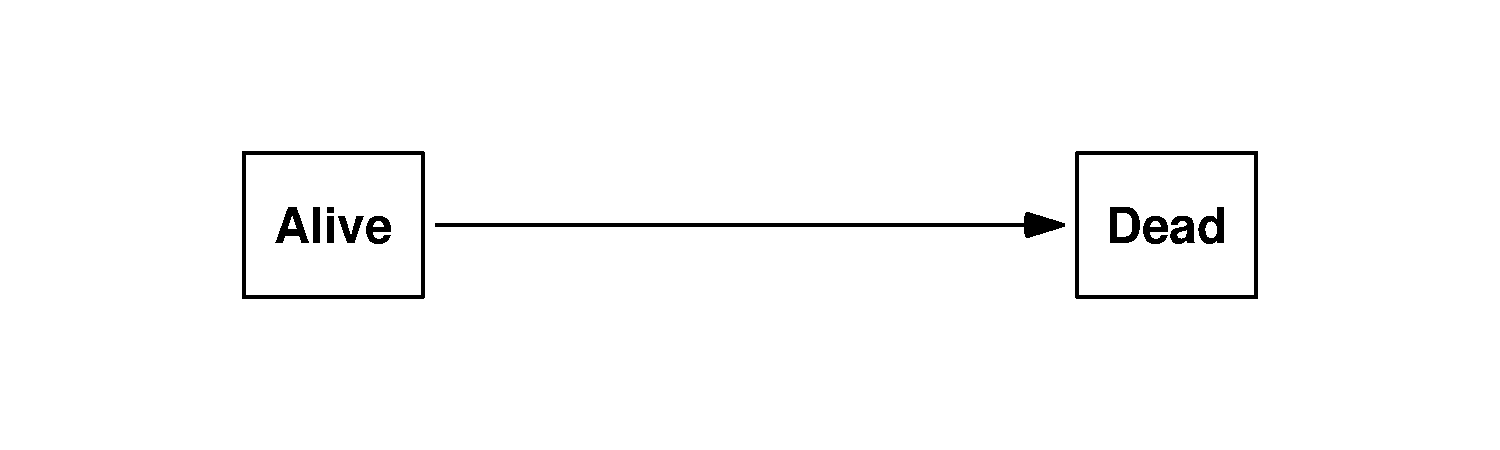
\includegraphics[width=\textwidth,keepaspectratio]{simple-surv}
%   \end{center}
% \end{frame}

%----------------------------------------------------------------------
\begin{frame}{Markov models for multistate diseases}
  The natural generalization of Poisson regression to multiple
    disease states:
  \pause
    \begin{itemize}
    \item Probability of transition between states depends \textbf{only} on current state
    \item --- this is the \textbf{Markov} property
    \item $\Rightarrow$ transition rates are constant over time
    \item (time-fixed) covariates may influence transition rates
    \item the formal Markov property is \textbf{very} restrictive
    \item In clinical litterature ``Markov model'' is often used
      about any type of multistate model
    \end{itemize}
\end{frame}

% %----------------------------------------------------------------------
% \begin{frame}{An Illness-Death Model}
% \vspace*{-1em}
% \hspace*{-2em}
% 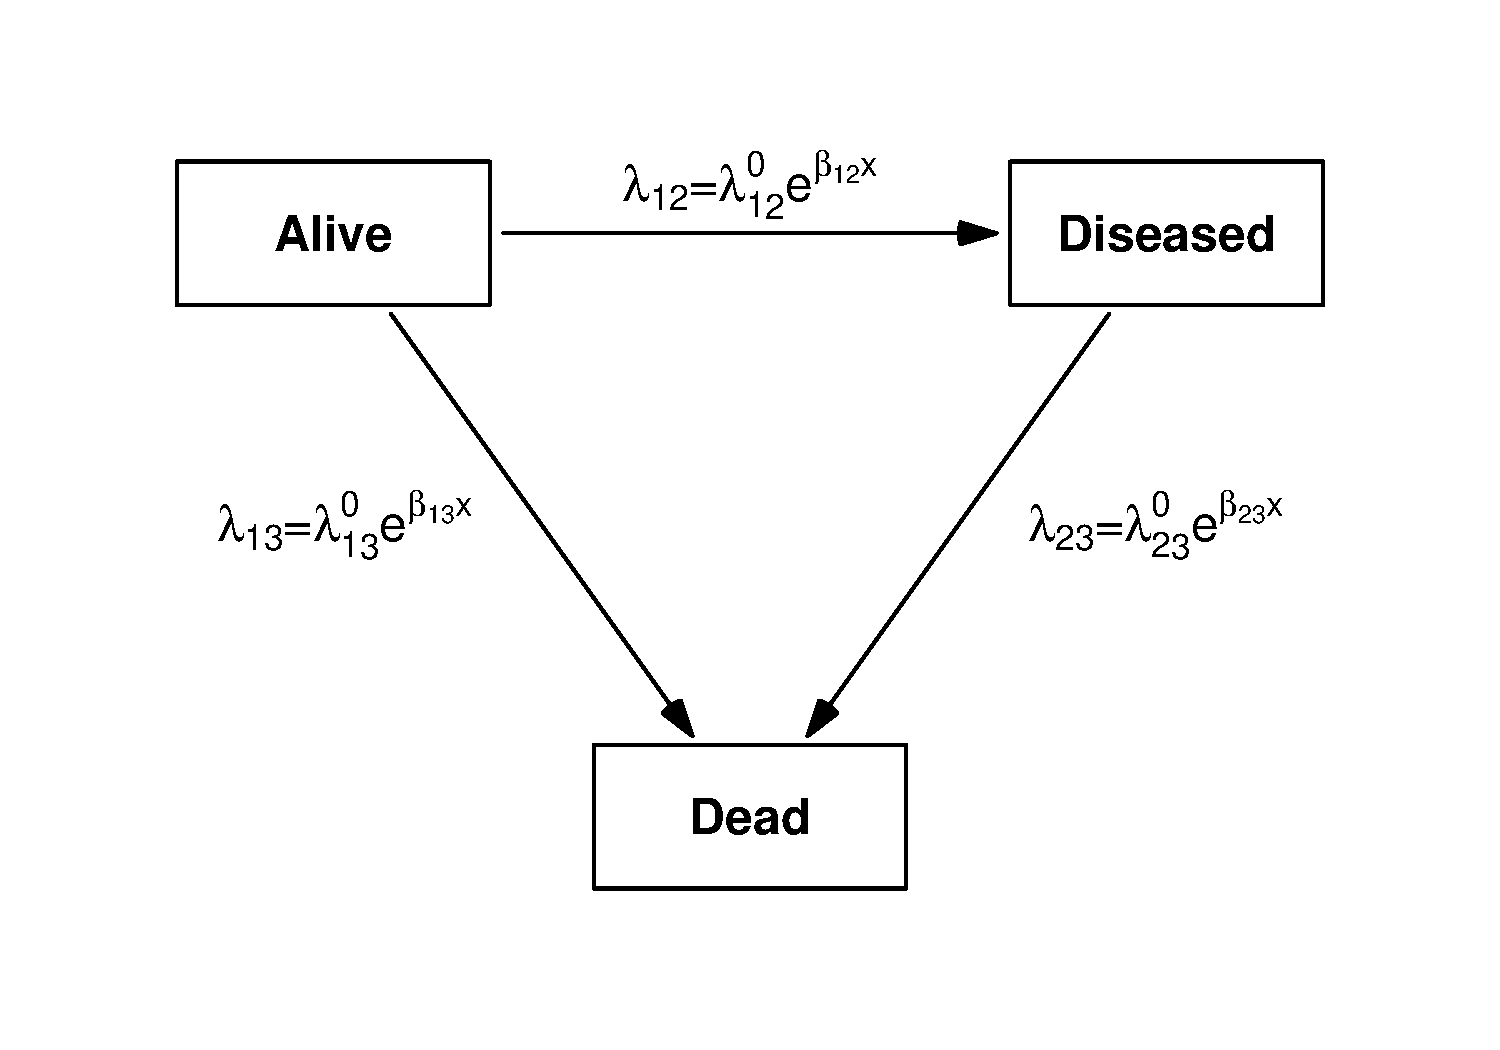
\includegraphics[height=0.85\textheight,keepaspectratio]{ill-death}\\[-1ex]
% Note: Constant transition intensities between states
% \end{frame}

%----------------------------------------------------------------------
\begin{frame}{Compnents of a multistate (Markov) model}
  \begin{itemize}
    \item Define the disease states.
    \item Define which transitions between states are allowed.
    \item Select covariates influencing transition rates (may be
      different between transitions)
    \item Constrain some covariate effects to be the same, or zero.
    \item Not a trivial task --- do we want \textit{e.g.}

      \begin{itemize}
      \item cause of death
      \item disease status at death
      \end{itemize}

  \end{itemize}
\end{frame}

\section{Defining Multi-State Markov Models}

% %----------------------------------------------------------------------
% \begin{frame}{Formal definition}
%   A model is defined by its \alert{transition intensity matrix}
%   \[
%   Q = \left(
%   \begin{array}{@{\extracolsep{1em}}ccc}
%     -\lambda_{12}  - \lambda_{13} & \lambda_{12}  & \lambda_{13} \\
%     0                            & -\lambda_{23} & \lambda_{23} \\
%     0                            & 0            &  1 \\
%   \end{array}
%   \right)
%   \]
%   \vspace*{-1em}
%   \pause
%   \begin{itemize}
%   \item Off-diagonal elements are instantaneous transition rates
%     (or intensities) between two different states.
%   \item If states are ordered by severity:

%     \begin{itemize}
%     \item Above the diagonal = progression
%     \item Below the diagonal = regression
%     \end{itemize}

%   \item Diagonal elements are fixed by the constraint that rows of $Q$
%     sum to zero.
%   \end{itemize}
% \end{frame}

%  %----------------------------------------------------------------------
% \begin{frame}{Likelihood for a Markov model}
%   \begin{itemize}
%   \item The likelihood of the model depends on the probability of being in
%     state $j$ at time $t_1$, given that you were in state $i$ at time $t_0$.
%   \item This is given by $P_{ij}$ where
%     \[
%     P = \exp(Q(t_1 - t_0))
%     \]
%   \item The \alert{matrix exponential} is hard to calculate (from a
%     numerical point of view).
%   \item \textbf{Only} refers to transition rates that are constant in time.
%   \end{itemize}
% \end{frame}

% %----------------------------------------------------------------------
% \begin{frame}
%   \frametitle{Covariate Effects are Multiplicative}

%   For an individual $i$ with risk factors $z_i$
%   \[
%   \lambda^i_{jk} = \lambda^0_{jk} \times \exp(\beta_{jk}^T z^i)
%   \]
%   There is a separate baseline rate hazard ratio for each possible
%   transition.
% \end{frame}

% %----------------------------------------------------------------------
% \begin{frame}
%   \frametitle{Hidden Markov Models}

%   For cases where the disease process is observed indirectly.
%   \pause
%   We have:
%   \begin{itemize}[<+->]
%   \item A possibly misclassified diagnosis, or
%   \item An indirect surrogate of disease status.
%   \end{itemize}
%   \pause
%   Add a \alert{measurement model} to describe the relation between
%   true and observed state.
%   \[
%   \mbox{P}(\mbox{Observed state} \mid \mbox{True state})
%   \]
% \end{frame}

%----------------------------------------------------------------------
\begin{frame}{Likelihood for multistate model}
  \begin{itemize}
  \item The likelihood of the model depends on the probability of being in
    state $j$ at time $t_1$, given that you were in state $i$ at time $t_0$.
  \item Assume transition rates constant in small time intervals
  \item $\Rightarrow$ each interval contributes terms to
    the likelihood:

    \begin{itemize}
    \item one for each person at risk of a transition in the interval
    \item \ldots for each possible transition
    \item each term has the form of a Poisson likelihood contribution
    \item the total likelihood for each time interval is a product of
      terms over persons and (possible) transitions
    \end{itemize}

  \item Total likelihood is product of terms for all intervals
  \item --- components \textbf{not} independent, but the total
    likelihood is a product; hence of the same form as the
    likelihood of independent Poisson variates
  \end{itemize}
\end{frame}

%----------------------------------------------------------------------
\begin{frame}{Purpose of multistate modeling}
  \begin{itemize}
  \item Separation of intensities of interest (model definition)
  \item Evaluation of covariate effects on these
  \item --- biological interpretability of covariate effects
  \item Use a fitted model to compute:
  \item state occupancy probabilities: $\ptxt{in state
      $X$ at time $t$}$
  \item time spent in a given state
  \end{itemize}
\end{frame}

%----------------------------------------------------------------------
\begin{frame}{Special multistate models}
  \begin{itemize}
  \item If all transition rates depend on only one time scale
  \item --- but possibly different (time-fixed) covariates
  \item $\Rightarrow$ easy to compute state probabilities
  \item For this reason the most commonly available models
  \item but not the most realistic models.
  \item Realistically transition rates depend on:
    \item multiple time scales
    \item time since entry to certain states.
  \end{itemize}
\end{frame}
